\documentclass[t, screen, aspectratio=43]{beamer}
\usepackage[T1]{fontenc}
\usepackage[utf8]{inputenc}
\usepackage{epsf}
\usepackage{graphicx}
\usepackage{geometry}
\usepackage{tabularx}
\usepackage[table]{colortbl}
\usepackage{xcolor}
\usepackage{soul}
% Use the NTNU-temaet for beamer 
% \usetheme[style=ntnu|simple|vertical|horizontal, 
%     language=bm|nn|en, 
%     smalltitle, 
%     city=all|trondheim|alesund|gjovik]{ntnu2017}
\usetheme[style=helvet,language=en]{ntnu2017}

\usepackage[english]{babel}
\usepackage[style=numeric,backend=biber,natbib=false,sorting=none]{biblatex}

\title[Short title]{Ultra-Low Power PLL for Wake-up Receiver Applications}
\subtitle{Specialization Project Progress - 5th Week}
\author[C Nielsen]{Cole Nielsen}
\institute[NTNU]{Department of Electronic Systems, NTNU}
\date{27 September 2019 (Week 39)}
%\date{} % To have an empty date

\addbibresource{example.bib} % Add bibliography database

% Set the reference style to numeric.
% See here: http://tex.stackexchange.com/questions/68080/beamer-bibliography-icon
\setbeamertemplate{bibliography item}[text] 

% Set bibliography fonts to a small size.
\renewcommand*{\bibfont}{\footnotesize}

\begin{document}

\begin{frame}
	\titlepage%
\end{frame}

% Alternatively, special title page command to get a different background
% \ntnutitlepage

% #############################################################################
% Timeline
% #############################################################################
\begin{frame}
	\frametitle{Autumn Timeline}
	\begin{table}[htb!]
		\tiny
		\centering
		\vspace{-1em}
		\def\arraystretch{1.5}		
		\setlength\arrayrulewidth{0.75pt}
		\setlength{\tabcolsep}{1em} % for the horizontal padding
		\begin{tabular}{|l|l|l|l|}
			\hline 
			\rule[-1ex]{0pt}{2.5ex} \cellcolor{gray!40}\textbf{Week Number} & \cellcolor{gray!40}\textbf{Dates} &\cellcolor{gray!40}\textbf{Tasks} & \cellcolor{gray!40}\textbf{Outcomes}\\ 
			\hline 
			\rule[-1ex]{0pt}{2.5ex} \cellcolor{red!20}\textbf{36}& \cellcolor{red!20}2.9 - 8.9 & \cellcolor{red!20}Review PLL Design & \cellcolor{red!20}Refreshed Knowledge\\ 
			\hline 
			\rule[-1ex]{0pt}{2.5ex} \cellcolor{red!20}\textbf{37}& \cellcolor{red!20}9.9 - 15.9 & \cellcolor{red!20}Modeling/simulation (set up) & \cellcolor{red!20}--\\ 
			\hline 
			\rule[-1ex]{0pt}{2.5ex} \cellcolor{red!20}\textbf{38}& \cellcolor{red!20}16.9 - 22.9 & \cellcolor{red!20}Modeling/simulation &\cellcolor{red!20} TDC/DCO Requirements\\ 
			\hline 
			\rule[-1ex]{0pt}{2.5ex} \cellcolor{green!20}\textbf{39}& \cellcolor{green!20}23.9 - 29.9& \cellcolor{green!20}Modeling/simulation& \cellcolor{green!20}Loop Filter/Digital Algorithms\\ 
			\hline 
			\rule[-1ex]{0pt}{2.5ex} \cellcolor{blue!20}\textbf{40}& \cellcolor{blue!20}30.9 - 6.10& \cellcolor{blue!20}Modeling/simulation& \cellcolor{blue!20}\color{red}{\textbf{Loop filter,}} \color{black}{Ideal implementation in Cadence}\\ 
			\hline 
			\rule[-1ex]{0pt}{2.5ex} \textbf{41}& 7.10 - 13.10& Circuit Research & DCO/Divider topologies\\ 
			\hline 
			\rule[-1ex]{0pt}{2.5ex} \textbf{42}& 14.10 - 20.10& Circuit Research & TDC/other topologies\\ 
			\hline 
			\rule[-1ex]{0pt}{2.5ex} \textbf{43}& 21.10 - 27.10& Circuit Implementation& Digital logic (schematic)\\ 
			\hline 
			\rule[-1ex]{0pt}{2.5ex} \textbf{44}& 28.10 - 3.11& Circuit Implementation& DCO (schematic)\\ 
			\hline 
			\rule[-1ex]{0pt}{2.5ex} \textbf{45}& 4.11 - 10.11& Circuit Implementation& Divider/other (schematic)\\ 
			\hline 
			\rule[-1ex]{0pt}{2.5ex} \textbf{46}& 11.11 - 17.11& Circuit Implementation (TDC)& \\ 
			\hline 
			\rule[-1ex]{0pt}{2.5ex} \textbf{47}& 18.11 - 24.11& Circuit Implementation (TDC)& TDC (schematic)\\ 
			\hline 
			\rule[-1ex]{0pt}{2.5ex} \textbf{48}& 25.11 - 1.12& Full Circuit testing & Testbenches, find bugs, design fixes\\ 
			\hline 
			\rule[-1ex]{0pt}{2.5ex} \textbf{49}& 2.12 - 8.12& Full Circuit testing& Design Fixes/iteration\\ 
			\hline 
			\rule[-1ex]{0pt}{2.5ex} \textbf{50}& 9.12 - 15.12& --& --\\ 
			\hline 
		\end{tabular}
		\begin{flushleft}\textbf{Legend:} \colorbox{red!20}{\textbf{Done}} \colorbox{green!20}{\textbf{Current}}  \colorbox{blue!20}{\textbf{Revised}}
		% *I will write the report simultaneously with the work.
		\end{flushleft}
		% \caption{Assigned specifications for branch line hybrid design.}
		% \label{asgn_specs}
	\end{table}   
\end{frame}


% #############################################################################
% This week
% #############################################################################

\begin{frame}
	\frametitle{Timeline Tasks}
	\begin{block}{This week}
		\begin{itemize}
			\footnotesize
			\item \textbf{Primary:} Loop analysis, requirements definition.
			\begin{itemize}
				\footnotesize
				\item Design open loop filter design to meet closed loop requirements.
				\begin{itemize}
					\item Dependent on DCO properties ($k_{DCO}$, $f_0$, tuning range).
					\item Difference equation implementing discrete time 2nd order IIR filter.
				\end{itemize} 
				\item Datapath requirements (fixed-point resolution)
			\end{itemize} 
		\end{itemize}    
	\end{block}
	\begin{block}{Next week - \color{red} \textbf{Revised}}
		\begin{itemize}
			\footnotesize
			\item \textbf{Primary:} Ideal component PLL implementation in Cadence, \color{red} continue loop filter work.
			\begin{itemize}
				\footnotesize
				\item Ideal component PLL implementation is not a lot of work.
				\item Loop filter very critical, spend more time on this.
				\begin{itemize}
					\footnotesize
					\item Need to make Verilog description of loop filter for simulation in Cadence.
				\end{itemize}
			\end{itemize} 
		\end{itemize}    
	\end{block}
\end{frame}

% #############################################################################
% sim/modeling approach
% #############################################################################

\begin{frame}
	\frametitle{Loop Filter}
	\begin{block}{Original Attempt}
		\vspace{-.2em}
		\vspace{-0.5em}
		\center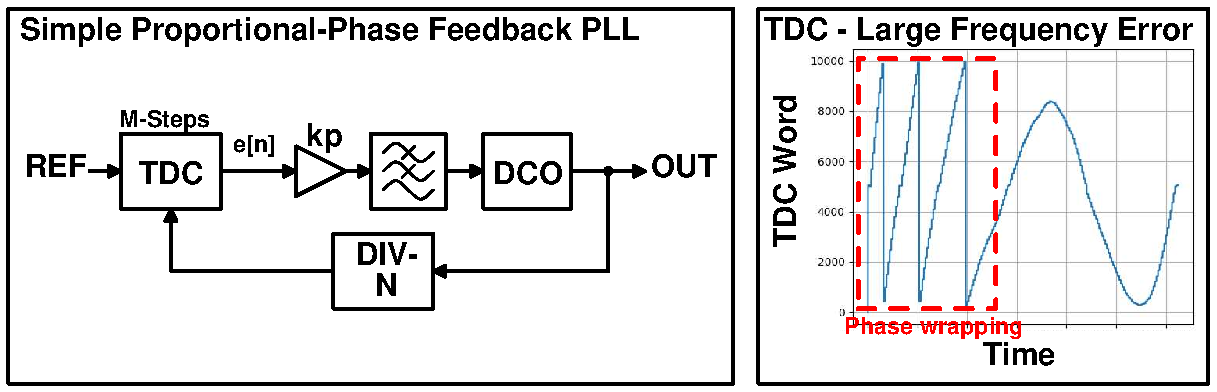
\includegraphics[width=0.75\textwidth, angle=0]{phase_wrap.pdf}
		\vspace{-0.5em}
		\begin{itemize}
			\footnotesize
			\item Started with simple PLL loop with proportional-phase fed into loop filter (LF).
			\begin{itemize}
				\scriptsize
				\item Not stable at large frequency offset, due to frequency wrapping. At the TDC:
				\tiny
				\begin{equation}
					\Delta \phi = \frac{2\pi \Delta f T}{N} \rightarrow T_{wrap} = \frac{N}{\Delta f}
				\end{equation}
				\scriptsize
				\item Upon cold start, $\Delta f$ is expected to be up to 100 MHz, N=150 $\rightarrow T_{wrap} = $ 1.5 $\mu$s
				\begin{itemize} 
					\scriptsize
					\item $f_{wrap} \sim$  600 kHz, this is unstable with a loop bandwidth of 100 kHz.
				\end{itemize}
				\item Must opt for alternate loop structure.
			\end{itemize}
		\end{itemize} 	
	\end{block}
\end{frame}


\begin{frame}
	\frametitle{Loop Filter}
	\begin{block}{New Approach}
		\vspace{-0.5em}
		\center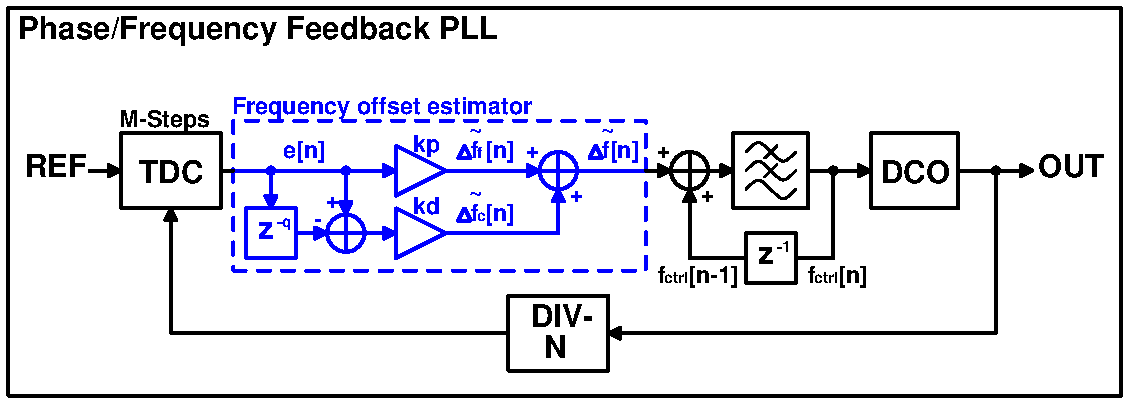
\includegraphics[width=0.75\textwidth, angle=0]{more_advanced.pdf}
		\vspace{-0.5em}
		\begin{itemize}
			\footnotesize
			\item Two-fold approach: utilize propotional-phase and coarse frequency offset estimation in feedback.
			\begin{itemize}
				\scriptsize
				\item Coarse frequency estimator to handle high frequency offset (e.g. cold start-up).	
				\item Proportional-phase for near steady state. Acts like fine frequency estimator.
			\end{itemize}
			\item Offset estimates are summed with previous oscillator tuning word (OTW, also $f_{ctrl}$ here), then low passed filtered to yield new OTW. 
			\begin{itemize}
				\scriptsize
				\item Low pass filter loop keeps steady state.	
				\item Frequency estimator updates if any changes detected.
			\end{itemize}			
		\end{itemize} 	
	\end{block}
\end{frame}

\begin{frame}
	\frametitle{Loop Filter}
	\begin{block}{Coarse frequency offset estimation}
		\vspace{-0.5em}
		\center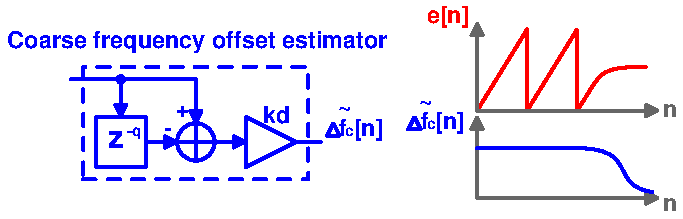
\includegraphics[width=0.5\textwidth, angle=0]{coarse_est.pdf}
		\begin{itemize}
			\footnotesize
			\item \textbf{Coarse frequency estimation:} Given M-step TDC, outputting phase error signal e$_\phi$[n], and a divider modulus N
			\tiny
			\vspace{-1em}
			\begin{equation}
				\Delta \phi_{DCO}[n; q] = N\cdot\Delta \phi_{REF}[n] = 2\pi \frac{N}{M}\left( e_\phi[n]-e_\phi[n-q]\right ),\hspace{2em} \Delta \phi_{DCO}[n; q] = \Delta \omega_{DCO}[n]qT_{ref} = 2\pi q \frac{\Delta \tilde f_{DCO}}{f_{ref}}
			\end{equation}
			\vspace{-1em}
			\begin{equation}
				\Delta \tilde f_{c} =\Delta \tilde f_{DCO} = \frac{f_{ref}}{q}\frac{N}{M}\left( e_\phi[n]-e_\phi[n-q]\right )
			\end{equation}				
			\footnotesize	
			\item Is a discrete differentiator, with gain coeficient to convert $d\phi/dt$ to frequency. 
			\begin{itemize}
				\scriptsize
				\item Design logic to handle phase wrapping.	
				\item Useful in coarse frequency range calibration. Can detect fast if frequency offset too large.
				\item Delay q is used to increase frequency resolution. 
			\end{itemize}			
		\end{itemize} 	
	\end{block}
\end{frame}


\begin{frame}
	\frametitle{Loop Filter}
	\begin{block}{Coarse frequency offset estimation - continued}
		\begin{itemize}
			\footnotesize
			\item Given DCO gain $K_{DCO}$, the required gain $K_d$ of the filter is:
			\tiny
			\vspace{-0.5em}
			\begin{equation}
				K_{d} = \frac{f_{ref}}{qK_{DCO}}\frac{N}{M}\left( e_\phi[n]-e_\phi[n-q]\right )
			\end{equation}				
			\footnotesize	
			\item Disable the coarse estimator if $e_\phi[n]-e_\phi[n-q]$ < some threshold:
			\begin{itemize}
				\scriptsize
				\item Offset small enough, allow to run as classical phase-detector mode.
			\end{itemize}	
		\end{itemize} 
	\end{block}
	\begin{block}{Fine frequency offset estimation}
		\begin{itemize}
			\footnotesize
			\item Proportional signal of phase error to estimate frequency error.
			\item Used in near-steady state. Loop will regulate to keep phase locked.
			\item Classical PLL operating mode.
		\end{itemize} 	
	\end{block}
\end{frame}


% \begin{frame}
% 	\frametitle{Loop Filter}
% 	\begin{block}{Modified implementation - PID}
% 		\vspace{-0.5em}
% 		\center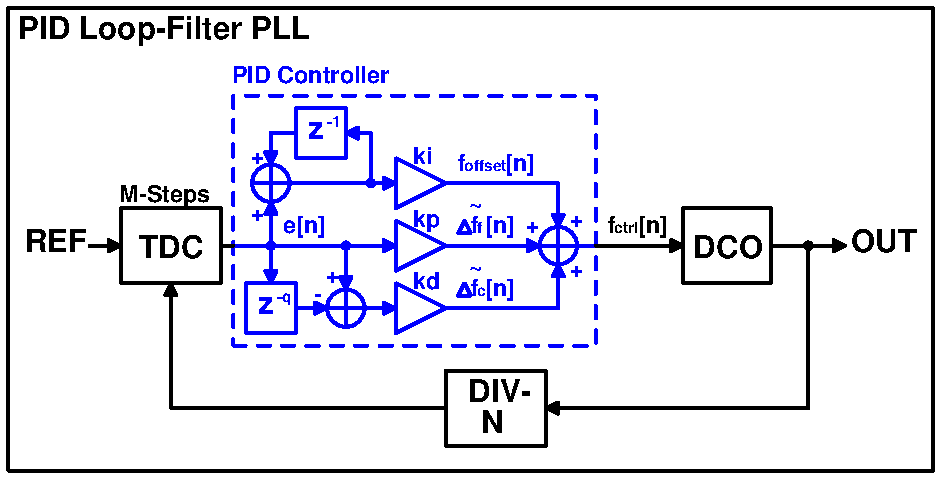
\includegraphics[width=0.5\textwidth, angle=0]{pid_pll.pdf}
% 		\vspace{-0.5em}
% 		\begin{itemize}
% 			\footnotesize
% 			\item On the observation that the loop filter was basically a PID controller.
% 			\begin{itemize}
% 				\scriptsize
% 				\item Add integral term to complete PID. Integral term keeps track of steady state offset of OTW, ideally yields 0 steady state error. 
% 				\item Derivative term \textit{only} used to perform coarse adjustment.
% 				\item Near/in steady, behaves as \textbf{PI controller}. 
% 			\end{itemize}
% 		\end{itemize} 	 
% 	\end{block}
% \end{frame}


\begin{frame}
	\frametitle{Loop Filter}
	\begin{block}{Loop Filter Gain Coefficients}
		\vspace{-0.5em}
		\center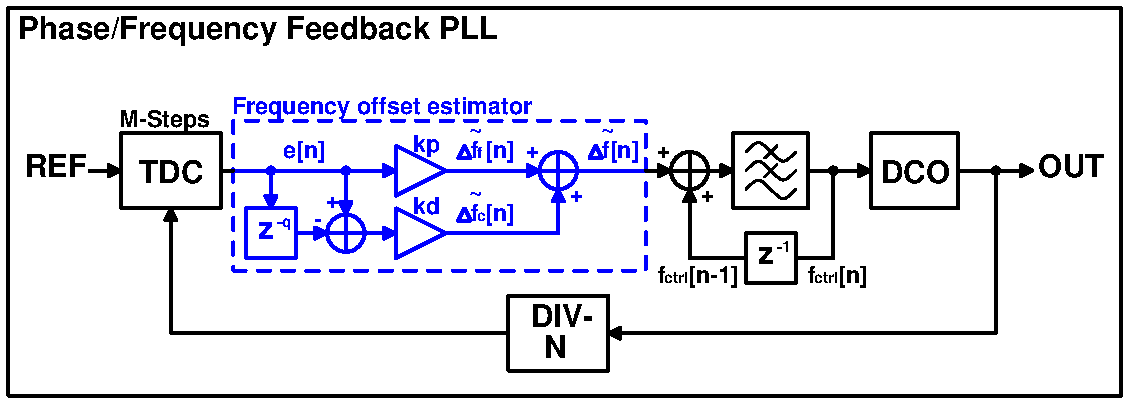
\includegraphics[width=0.75\textwidth, angle=0]{more_advanced.pdf}
		% \vspace{-0.5em}
		\begin{itemize}
			\footnotesize
			\item When running in proportional-only feedback mode, the open loop gain $A(f)$ is:
			\tiny
			\begin{equation}
				A(f) = K_p \frac{M}{N}\frac{K_{LPF}}{s + \omega_{LPF} - K_{LPF}}\frac{2\pi K_{DCO}}{s}
			\end{equation}
			\footnotesize
			\item The closed loop gain is therefore (continuous):
			\tiny
			\begin{equation}
				G(f) =  \frac{A(f)}{1+A(f)}= \frac{2\pi M K_pK_{LPF}K_{DCO}/N}{s^2+s(\omega_{LPF - K_{LPF}})/N + 2\pi M K_pK_{LPF}K_{DCO}/N}
			\end{equation}	
		\end{itemize} 	 
	\end{block}
\end{frame}

\begin{frame}
	\frametitle{Loop Filter}
	\begin{block}{Loop Filter Gain Coefficients}
		\begin{itemize}
			\scriptsize
			\item The form of a second order low pass filter is, with natural frequency $\omega_n$ and damping coefficient $\zeta$:
			\tiny
			\begin{equation}
				H_{LPF}(f) = \frac{\omega_n^2}{s^2 + 2\zeta\omega_ns + \omega_n^2}
			\end{equation}
			\scriptsize
			\item Setting $H_{LPF}(f) = G(f)$, equivalencies for $\omega_n$ and $\zeta$ are found:
			\tiny
			\begin{equation}
				\omega_n = \sqrt{2\pi M K_pK_{LPF}K_{DCO}/N}
			\end{equation}			
			\begin{equation}
				\zeta = \frac{\omega_{LPF - K_{LPF}}}{2\sqrt{2\pi MN K_pK_{LPF}K_{DCO}}}
			\end{equation}	
			\scriptsize
			\item The Butterworth closed loop response with 100 kHz bandwidth, $\omega_n \sim 2\pi\cdot 100 Khz$, $\zeta=0.707$.
			\item Coefficients $K_{LPF}$, $K_p$, $\omega_n$ can be solved computationally.
			\item Need to reformulate in Z-domain.
		\end{itemize} 	 
	\end{block}
\end{frame}

\begin{frame}
	\frametitle{Frequency Calibration}
	\begin{block}{Coarse frequency calibration algorithm}
		\begin{itemize}
			\vspace{-0.25em}
			\scriptsize
			\item Ring oscillator DCOs will have large variation in frequency due to PVT variation.
			\item Use bank of coarse capacitance values to correct range of oscillator.
			\item Coarse frequency estimator used in this calibration.  DCO is has a fine range of $\Delta f_{fine}$.
		\end{itemize} 	
		\vspace{-0.25em}
		\scriptsize
		\textbf{Coarse frequency tuning state machine} (as pseudo-code)
			\begin{enumerate}
				\scriptsize
				\item $C_{tune}$ = $C_{opt}$ = 0;\hspace{1em} LE = $\Delta f_{fine}$		
				\item Reset PLL
				\item Estimate Frequency offset $\rightarrow \tilde f_{offset}$
				\vspace{-0.2em}
				\item \textbf{If} abs($\tilde f_{offset}$ - $\Delta f_{fine}/2$)  \textbf{<} LE: \hspace{1em}\color{teal} // Centers fine tuning range around target frequency
				\color{black}
				\begin{itemize}
					\scriptsize
					\item LE = abs($\tilde f_{offset}$ - $\Delta f_{fine}/2$)
					\item $C_{opt}$ = $C_{tune}$
				\end{itemize}	
				\item \textbf{If} $C_{tune}$ \textbf{==} $C_{max}$: \textbf{Goto} 8		
				\item $C_{tune}$ += 1
				\item \textbf{Goto} 2
				\item $C_{tune}$ = $C_{opt}$; \textbf{End}
			\end{enumerate}
 
	\end{block}
\end{frame}


% #############################################################################
% Loop Dynamics (continuous)
% #############################################################################

% \begin{frame}
% 	\frametitle{Loop Dynamics}
% 	\begin{block}{Still To Do}
% 		\vspace{-.2em}
% 		\begin{itemize}
% 			\footnotesize
% 			\item Standard approach to used mixed continuous/discrete time mathematical model for DPLL. 
% 			\item Plot of RO phase noise (typical)
% 			\item Automatic analysis of performance (lock detection, residual phase modulation, lock-in/pull-in range).
% 			\item Automatic optimization (using gradient descent) of PLL parameters?
% 			\item Z-domain modeling of loop? Develop (by hand) some ideal transfer funtions for loop.

% 		\end{itemize}    
% 	\end{block}
% \end{frame}

% #############################################################################
% Specification
% #############################################################################

\begin{frame}
	\frametitle{Specification (unchanged)}
	\begin{block}{System Performance Targets}
		\scriptsize
		\begin{table}[h!]
			\centering
			\def\arraystretch{1.5}		
			\setlength\arrayrulewidth{0.75pt}
			\setlength{\tabcolsep}{1em} % for the horizontal padding
			\begin{tabular}{|l|r|l|l|}
				\hline 
				\rule[-1ex]{0pt}{2.5ex} \cellcolor{gray!40}\textbf{Parameter} & \cellcolor{gray!40}\textbf{Value} & \cellcolor{gray!40}\textbf{Unit }& \cellcolor{gray!40}\textbf{Notes}\\ 
				\hline 
				\rule[-1ex]{0pt}{2.5ex} \textbf{Frequency}  & 2.4-2.4835 & GHz & 2.4G ISM Band\\ 
				\hline 
				\rule[-1ex]{0pt}{2.5ex} \textbf{Ref. frequency} & 16 & MHz & Yields 6 channels \\ 
				\hline 
				\rule[-1ex]{0pt}{2.5ex} \textbf{Power} & $\leq$ 100  &$\mu$W & \\ 
				\hline 
				\rule[-1ex]{0pt}{2.5ex} \textbf{Residual FM} & $\leq$ 107  &kHz$_{RMS}$ & BER $\leq$ 1e-2, $f_{dev}$=$\pm$250 KHz\\ 
				\hline 
				\rule[-1ex]{0pt}{2.5ex} \textbf{Initial Lock Time} & $\leq$ 50 & $\mu$s & Upon cold start \\ 
				\hline 
				\rule[-1ex]{0pt}{2.5ex} \textbf{Re-lock Time} & $\leq$ 5 & $\mu$s & Coming out of standby \\ 
				\hline 
				\rule[-1ex]{0pt}{2.5ex} \textbf{Bandwidth} & 100 & kHz & (nominally), tunable \\ 
				\hline 
			\end{tabular} 
			% \caption{Assigned specifications for branch line hybrid design.}
			% \label{asgn_specs}
		\end{table}   
		Additionally: PLL output should support IQ sampling at LO frequency.
	\end{block}    
\end{frame}

\begin{frame}
	\frametitle{Specification (new)}
	\begin{block}{PLL Component Performance Targets}
		\scriptsize
		\begin{table}[h!]
			\centering
			\def\arraystretch{1.5}		
			\setlength\arrayrulewidth{0.75pt}
			\setlength{\tabcolsep}{1em} % for the horizontal padding
			\begin{tabular}{|l|r|l|l|}
				\hline 
				\rule[-1ex]{0pt}{2.5ex} \cellcolor{gray!40}\textbf{Parameter} & \cellcolor{gray!40}\textbf{Value} & \cellcolor{gray!40}\textbf{Unit }& \cellcolor{gray!40}\textbf{Notes}\\ 
				\hline 
				\rule[-1ex]{0pt}{2.5ex} \textbf{DCO LSB Resolution}  & $\leq$ 50  & kHz & Determined from quantization noise.\\ 
				\hline 
				\rule[-1ex]{0pt}{2.5ex} \textbf{DCO DNL} & < 1 & LSB & Ensures monotonicity \\ 
				\hline 
				\rule[-1ex]{0pt}{2.5ex} \textbf{TDC Resolution} & $\leq$ 3.8  & ns & \\ 
				\hline 
				\rule[-1ex]{0pt}{2.5ex} \textbf{TDC Resolution (bits)} & $\geq$ 4.03 &bits & \\ 
				\hline 
			\end{tabular} 
			% \caption{Assigned specifications for branch line hybrid design.}
			% \label{asgn_specs}
		\end{table}   
	\end{block}    
\end{frame}

% #############################################################################
% Architecture - block diagram
% #############################################################################

\begin{frame}
	\frametitle{Architecture (unchanged)}
	\begin{block}{Block Diagram}
	\center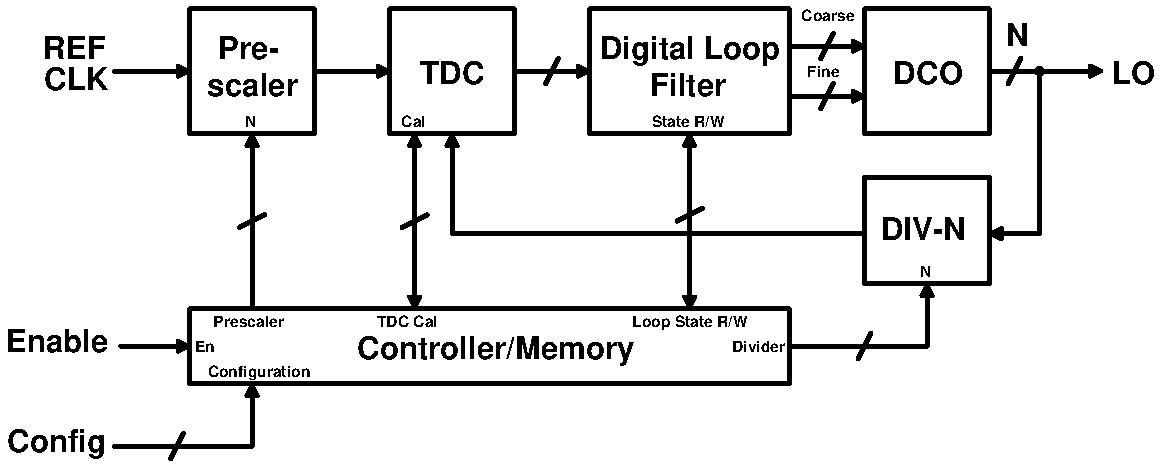
\includegraphics[width=0.75\textwidth, angle=0]{pll2.pdf}

	\end{block}
		\begin{block}{Power Targets}
		\vspace{-.1em}
		\begin{table}[htb!]
			\tiny
			\centering
			\def\arraystretch{1.5}		
			\setlength\arrayrulewidth{0.75pt}
			\setlength{\tabcolsep}{1em} % for the horizontal padding
			\begin{tabular}{|l|l|l|l|l|}
				\hline 
				\rule[-1ex]{0pt}{2.5ex} \cellcolor{gray!40}\textbf{DCO} & \cellcolor{gray!40}\textbf{TDC} & \cellcolor{gray!40}\textbf{Divider }& \cellcolor{gray!40}\textbf{Other} & \cellcolor{gray!40}\textbf{SUM} \\ 
				\hline 
				\rule[-1ex]{0pt}{2.5ex} 70 $\mu$W& 20 $\mu$W & 10 $\mu$W & $<<$ 1 $\mu$W & 100 $\mu$W\\ 
				\hline 
			\end{tabular} 
			% \caption{Assigned specifications for branch line hybrid design.}
			% \label{asgn_specs}
		\end{table}   
	\end{block}

\end{frame}


% #############################################################################
% project phases
% #############################################################################


\begin{frame}
	\frametitle{Project Phases}
	\begin{block}{Autumn 2019}
		\footnotesize
		\begin{itemize}
			\item System modeling and simulation.
			\begin{itemize}
				\footnotesize
				\item Learn PLL theory in detail
				\item Evaluate feasability of PLL architectures (counter, TDC-based)
				\item Determine requirements for TDC/DCO/Divider/logic (bits of resolution, accuracy etc) to meet PLL performance specifications.
				\item Determine digital logic for loop filter, validate stability and lock time performance.
			\end{itemize}
			\item Research ultra-low power circuit topologies to implement system components that will meet determined requirements.
			\item Translate component-level specifications into schematic-level circuit designs.
			\begin{itemize}
				\footnotesize
				\item Try, fail, try again until functional at schematic level.
				\begin{itemize}
					\footnotesize
					\item I expect the TDC to be difficult.
				\end{itemize}
			\end{itemize}      
		\end{itemize}
	\end{block}
\end{frame}

% #############################################################################
% Project phases slide 2
% #############################################################################


\begin{frame}
	\frametitle{Project Phases (continued)}
	\begin{block}{Spring 2020}
		\begin{itemize}
			\footnotesize
			\item Finalize schematic-level design.
			\item Estabilish thorough tests for PLL performance (automated?) to help in layout.
			\item Layout of PLL.
			\begin{itemize}
				\footnotesize
				\item Design iteration until design specs met.
				\item Probably very time consuming.
			\end{itemize}
			\item Full characterization/validation of design performance. 
			\begin{itemize}
				\footnotesize
				\item Comprehensive Corners/Monte-Carlo testing (time consuming??)
				\item More design iteration if new issues crop up...
			\end{itemize}
			\item Thesis paper writing.
		\end{itemize}
	\end{block}
\end{frame}

% #############################################################################
% References
% #############################################################################


% \begin{frame}
% 	\frametitle{Project Phases (continued)}
% 	\begin{block}{Spring 2020}
% 		[1] "Digital Frequency Synthesizers", Michael Perrott, 2019.\\
% 		\hspace{16pt}\url{http://www.cppsim.com/PLL_Lectures/day4_am.pdf}\\
% 		\vspace{1em}
% 		[2] "Minimum Achievable Phase Noise of RC Oscillators",
% 	Navid et al. 2005
% 	\end{block}
% \end{frame}


\end{document}
